\chapter{Usability study}

In this paper I have so far described my first contribution: a design for manually clustering nodes and my second contribution a working prototype that implements those designs. My final contribution in the field of provenance is a usability study to evaluate learnability, ease of use, efficiency, recovery from errors and user attitude towards my prototype. I particularly felt that this was a requirement for designing an interface because unless an interface is usable it can not be useful. Below I go into details about the design of the study then in the next section I discuss the results.

\section{Study Design}
\label{sec:study_design}

\label{sec:interview_format}

I decided to conduct a think aloud study with participants while using the ProvOwl application. A think aloud involves having a user try to accomplish a set of tasks whilst you watch and take notes. Jakob Nielsen, a researcher specialising in discount usability engineering, describes it as the following:

\begin{quote}
``In a thinking aloud test, you ask test participants to use the system while continuously thinking out loud — that is, simply verbalizing their thoughts as they move through the user interface.'' 
\end{quote}

Participants are encouraged to ``think aloud'' as they complete tasks to give incite into what they are thinking. I selected this approach for a number of reasons. Firstly, it has been used successfully for a long time. \citeauthor{nielsen1994} describes it as ``...the single most valuable usability engineering method.'' in his 1993 book \citetitle{nielsen1994}~\cite{nielsen1994}. Secondly, it requires a small number of users to get meaningful results. A post written in 2012 by \citeauthor{nielsen1994} describes why you only need to test with five users\footnote{Thinking Aloud: The \#1 Usability Tool: \url{https://www.nngroup.com/articles/thinking-aloud-the-1-usability-tool/}}. And lastly, I have conducted think aloud studies previously, so they are a natural first thought to me when gauging how usable an interface is.

Below I discuss the general format of the interviews and then in detail each of the scenarios users undertook and the tasks associated with each. The entire questionnaire I used for conducting the interviews can be seen at \ref{sec:interview_questionnaire}.


\subsection{Interview format}

The interviews were undertaken wherever was most convenient to the participant, this included at my desk, at the participants house or at coffee shops. The participants were asked a series of background questions, then undertook three scenarios in a think aloud study and finally were asked to complete a system usability scale questionnaire.

\subsubsection{Background Information}
\label{sec:background_information}

General background information was collected about each participant. Gender, age group and highest level of education. These were recorded in order to identify any demographic skew that I may have in my cohort as well as in case any unexpected correlations occurred. The last question in this background survey asked if the participant had heard of the term \textit{provenance} before, and if so to explain what it meant. Because provenance is used in other fields (such as accounting and art dealership) I wanted to identify anyone who had previous concepts of provenance and lineage to identify if this effected their ability to interpret provenance graphs.

\subsubsection{scenarios}

After the participant had answered the general background questions they were given a information sheet that explained the concept of provenance and showed an example of a provenance graph, explaining what each of the different coloured and shaped nodes meant (\ref{sec:prov_primer}). This allowed participants to have a uniform understanding of the concept of provenance regardless of whether they had heard of it before. Notes were taken of any questions the participant had whilst reading the information sheet.

They were then given my laptop. If the participant was not used to using a touchpad they were also supplied with a USB mouse. Open in a full screen browser was three tabs, one for each scenario the participant had to complete. Each scenario then has a series of tasks they had to either answer or complete, in some cases users required prompting to complete a task, in these cases I noted that the task was completed but with help. Each of the scenarios and tasks are discussed in detail in Section~\ref{sec:scenarios}.

\subsubsection{SUS Questionnaire}
\label{sec:sus_questionnaire}

The System Usability Scale has been around since 1996 when it was described by \citeauthor{brooke1996} in the paper \citetitle{brooke1996}~\cite{brooke1996} and provides a quick easy way of identifying if an interface is easy to use or not. It consists of 10 questions each requiring a response on a scale of 1--5. Users are asked to reply with what they intuitively feel rather than thinking about the questions for an extended period. 

I decided to use the SUS questionnaire because it is easy to administer (takes less than five minutes for users to complete), is valid in differentiating between usable and unusable interfaces~\cite{sauro2011} and can be used on a small sample size with reliable results\footnote{The usability.gov website has a good description of what a SUS questionnaire is and how to use it: https://www.usability.gov/how-to-and-tools/methods/system-usability-scale.html}.

\subsubsection{Coded questions}
\label{sec:coded_questions}

Each question was given a set of points, user actions that could be checked off if a user did them. For example, in question one of exercise one, the participant was asked \textit{What infroation is used to calculate your [fitness] score?}. One of the points for this question was \textit{ungrouped nodes}, so if the user ungrouped nodes while answering the question this point was ticked off. Whilst hand written notes were also taken during interviews, these checkboxes made for an easy way of identitying what common actions users undertook to complete exercises. 

Each point was assigned a code identifying what class of activity it belonged to. In the above example the ungrouping point had the code \textit{grouping-ungroup} because it's completing a grouping function and in particular an ungrouping function. 

Each of the codes are listed in Table~\ref{tab:question-codes} (page~\pageref{tab:question-codes}) with an explanation of the user behaviour they map to.

\subsection{Scenarios}
\label{sec:scenarios}

The user was asked to undertake three different scenarios, each with its own provenance file and a set of related tasks. Using multiple scenarios allowed me to have tasks that focussed on different objectives, for example the first scenario focuses on provenance understanding whilst the second and third are on provenance modification.

\subsubsection{Scenario 1: Alice's Fitness Score}
\label{ssub:scenario_1_alice_s_fitness_score}

In the first scenario the user is asked to imagine that they're Alice, they track their fitness information with a Fitbit for steps and a Withings scale for weight (images were shown to describe these objects as seen in \ref{sec:information_sheet}). The full paragraph given to participants:

\begin{framed}
Suppose you are Alice. You have been using your FitBit and Withings scales for 3 years to reduce your weight to 61kg and to increase your physical activity to 8000 steps a day. You have just linked your FitBit account to two friends, Bob and Carol. Recently FitBit introduced a fitness score that is shared and ranked with your friends\textellipsis This makes you wonder just how your score has been calculated.
\end{framed}

They were then asked to complete the following tasks, all of which required only a verbal answer.
\begin{enumerate}[label=\arabic*.]
	\item What data about you is used to calculate your score?
	\item Identify what aspects of the provenance graph map to your fitness dashboard.
	\item What processes does your raw step data go through before been used to calculate the fitbit\_score?
	\item How do you expect your raw fitbit data would be represented once it got to score\_generator?
	\item What processes does your Withings scale data go through before been used to calculate the fitbit\_score?
	\item How do you expect your weight data would be represented once it got to score\_generator?
	\item Are you concerned about how you data is used to calculate the fitbit score. Explain your reasoning. 
\end{enumerate}

The provenance graph they were given to answer these tasks can be seen in Figure~\ref{fig:exercise1a}. It can be seen from the light blue circles that this included composite nodes. I did this so that users were required to uncluster nodes (either by double clicking or selecting ``ungroup'' from the contexual commands) in order to properly answer the tasks. This meant that users were introduced to the idea of clustering before having to create them themselves in later tasks. These tasks also allowed the user to get used to reading provenance graphs. Questions 3,4 and 5,6 mirror each other so that if the user had difficulty understanding the way lineage worked in tasks 3,4, requiring prompting, they could then accomplish 5,6 on their own. The last question 7 was simply a way of gauging what users found important, whether they where concerned about privacy or transparency in calculations.

This scenario was purely exploration based and no modifications of the graph where required in order to complete the tasks.

\begin{figure}[h]
	\begin{subfigure}[t]{0.4\textwidth}
	\centering
	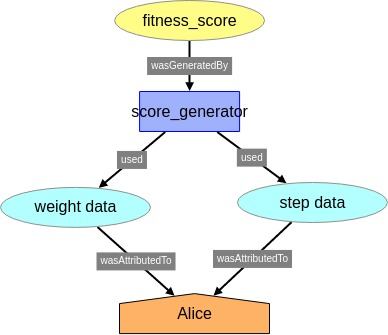
\includegraphics[width=\linewidth]{exercise1a}
	\caption{Alice's fitness score provenance with clusters.}
	\label{fig:exercise1a}
	\end{subfigure}
	\begin{subfigure}[t]{0.4\textwidth}
	\centering
	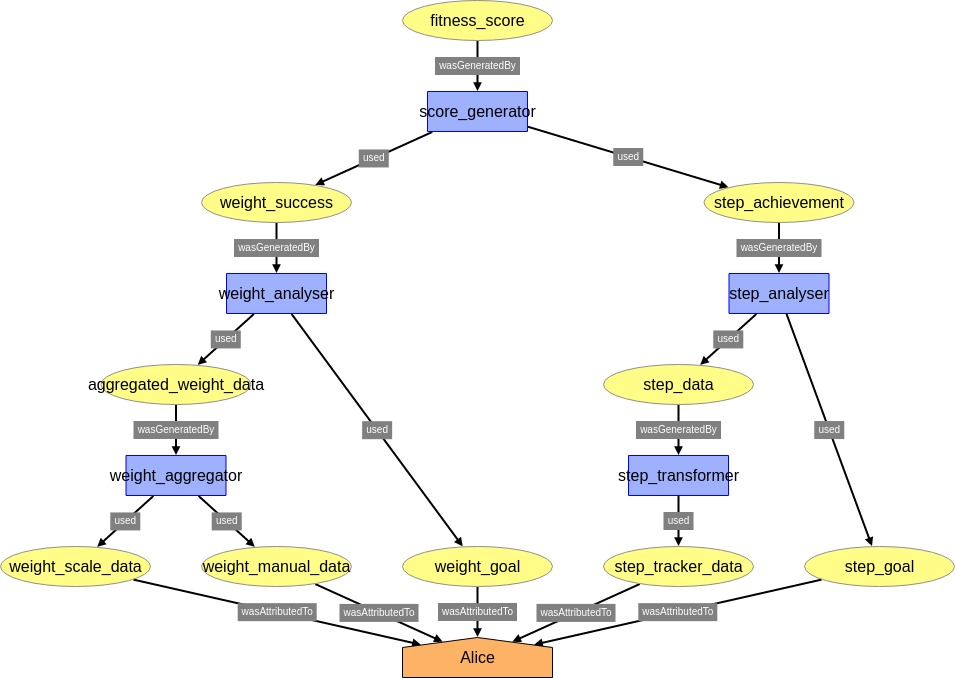
\includegraphics[width=\linewidth]{exercise1b}
	\caption{Alice's fitness score provenance without clusters.}
	\end{subfigure}
	\caption{The provenance graph used in scenario one showing the lineage of Alice's fitness score. The graph began with clusters as seen on the left. Completely unclustered the graph resembled that on the right.}
\end{figure}

\subsubsection{Scenario 2: Citizen Data Report}
\label{ssub:Scenario 2: Citizen Data Report}

The second exercise involved a larger amount of data and asked participants to imagine themselves as the curator of a citizen science project. Data was been tracked about multiple users and then used in a report that gave feedback on how to improve the cohorts overall fitness. The full paragraph given to participants was:

\begin{absolutelynopagebreak}
\begin{framed}
You are a researcher creating a citizen-data-report that recommends strategies for improving the fitness of your local community. You have step, location, weight and calorie information about members of the community. You are using this information to create multiple reports regarding fitness and weight information which will be used to support a final report addressed to the community on strategies that can be used to improve overall fitness. 
\end{framed}
\end{absolutelynopagebreak}

They were then asked to compete the following tasks. 

\begin{enumerate}[label=\arabic*.]
	\item Describe the graph to me
	\item You want to share how the report was generated with a colleague however you want to hide information about the cohort for privacy. Modify the graph in order to hide identifying information about participants. Then save an image of it. Note: try using the filter function for grouping multiple nodes
	\item You want to show Alice how her information is been used by sharing an image of the provenance with her that illustrates the lineage of the citizen report and how her data influences it. You don’t want Alice to see details about other people in the cohort. 
\end{enumerate}

The first task just required that the user describe the graph verbally to me. This did two things: it let me check that the user was correctly interpreting the information stored in the graph as well as forcing users to study and understand the graph (in early tests of the study without this question users would make mistakes later because of poor understanding of the graph).

The second task required the user to cluster nodes and in some cases to rename nodes. This task focused on users \textit{hiding} information. It required 40 nodes to be clustered together so participants sometimes needed prompting towards using the search command. 

\begin{figure}[h]
	\centering
	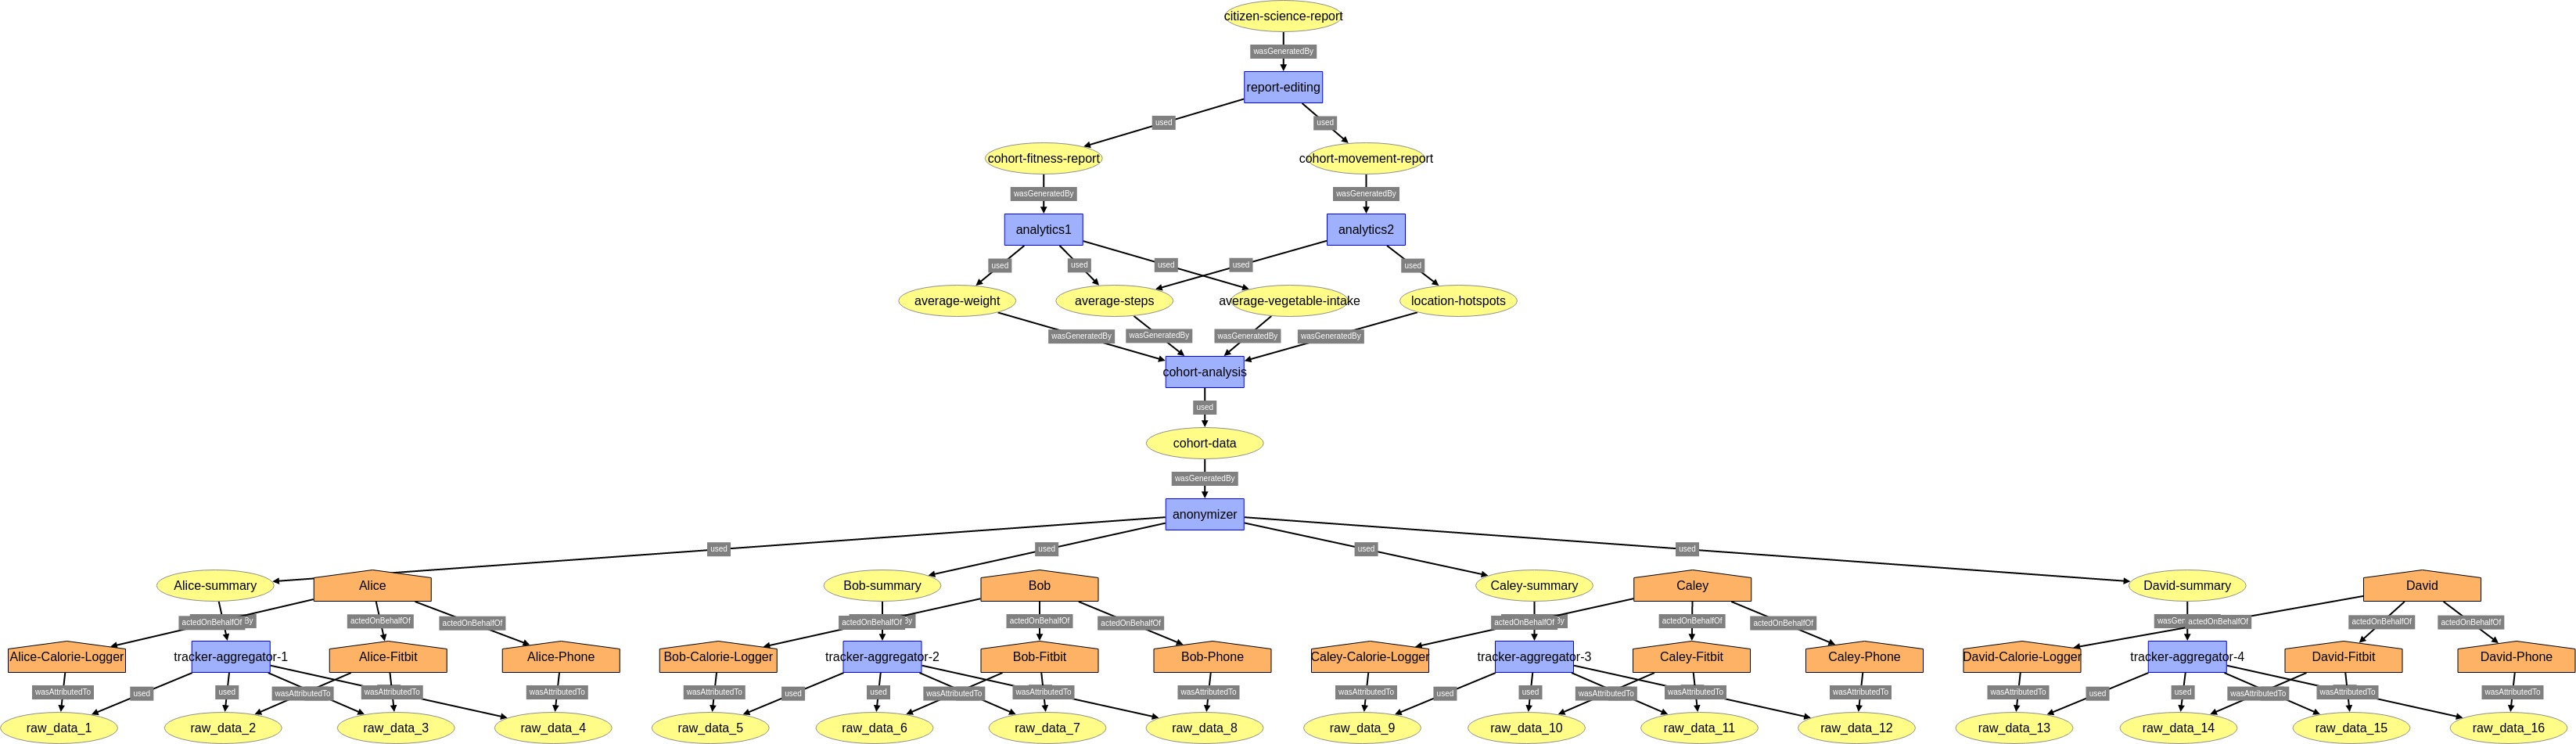
\includegraphics[width=0.8\linewidth]{exercise2}
	\caption{The provenance graph used in scenario 2 showing the lineage of a citizen science report. The top section of the graph is related to the report writing process whilst the fan out  at the bottom shows information stored about five different people.}
	\label{fig:exercise2}
\end{figure}


\subsubsection{Scenario 3: Twitter Data Report}
\label{ssub:Scenario 3: Twitter Data Report}

The third and final scenario was basically a duplicate of the second scenario on a more abstract provenance graph. It also focused on getting users to convey certain information through the graph rather than just hiding information. The provenance given to the user was that of a advice-report concerning information from multiple twitter feeds. The paragraph given to participants was: 

\begin{framed}
This provenance graph is an abstract representation of a report based on twitter data. 
\end{framed}

They were then asked to complete the following tasks:

\begin{enumerate}[label=\arabic*.]
	\item Describe the graph to me
	\item You want to modify the graph in order to convey the following information to a non-technical user: An advice report was created using data from 3 other reports based on twitter data from two different users. 
	\item You want to show to user X that their data was used in the advice report by sharing an image of the provenance with them. Modify the graph to best represent this information. 
\end{enumerate}

Same as scenario two the first task was used as a way of letting me check the user correctly understood the graph. The second and third tasks are a little different. They focus on asking the user to convey information by simplifying the graph. Compared to scenario two the results of these tasks a much more different from user to user. This seems to be related to different people explaining things different ways, it seemed that people who read graphs a lot were happy to leave the graph (seen in Figure~\ref{fig:exercise3}) the way it was because they could easily read information from it. 

The reasoning behind having this scenario similar to scenario two is that if the user required a large amount of prompting the complete scenario two then this gives them a chance to complete a clustering task without the help of the supervisor. If the user had managed to successfully cluster in scenario two then we got information about how they conveyed information. 

\begin{figure}[h]
	\centering
	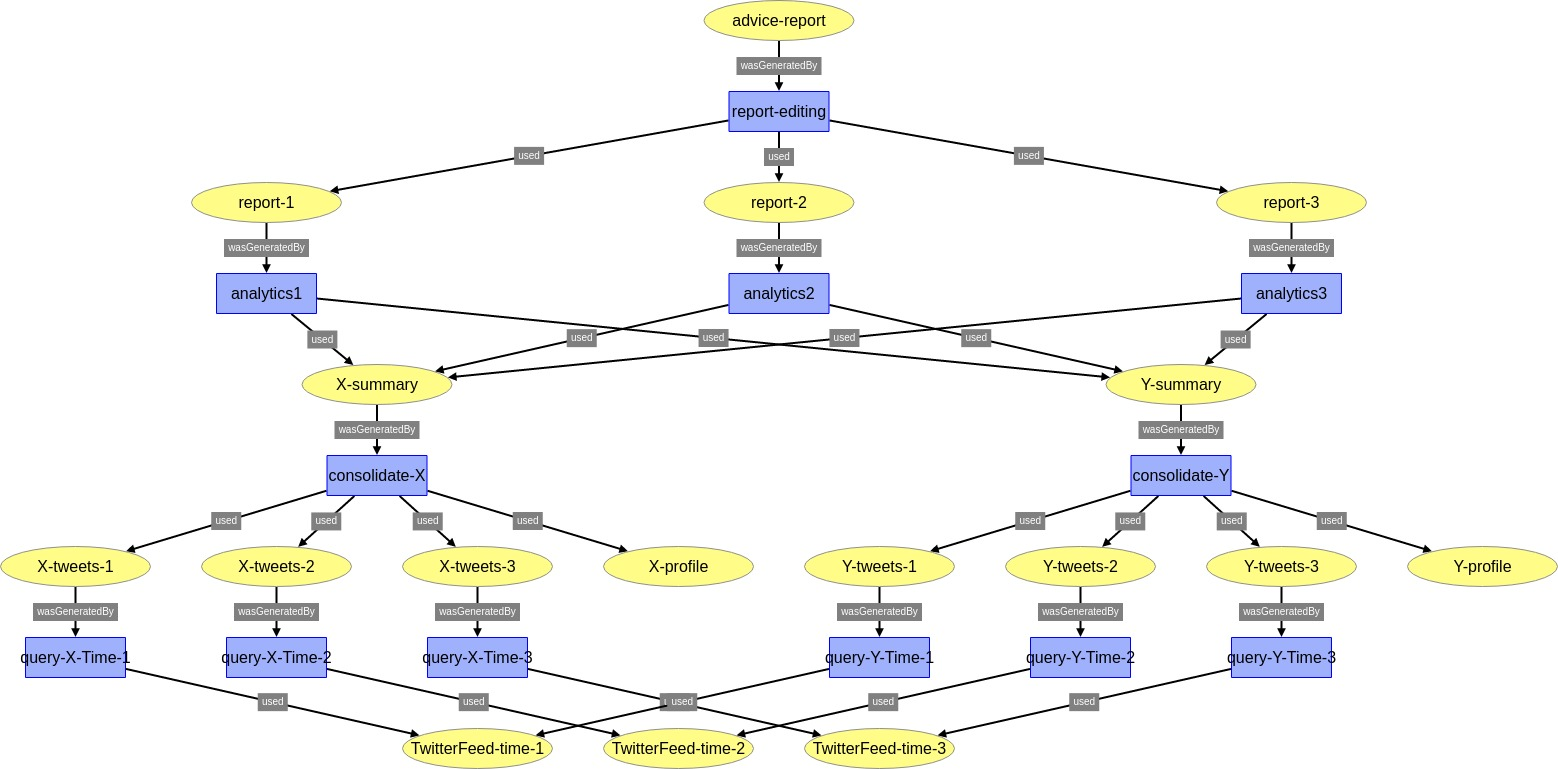
\includegraphics[width=0.8\linewidth]{exercise3}
	\caption{The provenance graph used in scenario 3 showing the lineage of a report on twitter data. This is a more abstract provenance graph and shows twitter data from three raw streams been analysed intro three reports and finally used in a single \textit{advice-report}.}
	\label{fig:exercise3}
\end{figure}

\subsection{Task Coding}
\label{sub:coding_tasks}

To help with analysing the results from the think aloud study the tasks were coded to represent what \textit{conceptual} activity and \textit{concrete} actions the user was expected to perform. 

The coding was used to identify what high level activity the user was accomplishing, for example if the task asked to trace the lineage of an entity this would accomplish the conceptual activity of \textit{identifying lineage}. There was five conceptual tasks the user had to perform to complete all the tasks: \textit{Understanding lineage:} The user had to be able to understand how lineage flowed through a provenance graph. \textit{Un-clustering Nodes:} The under had to uncluster nodes. \textit{Cluster Nodes:} The user had to cluster nodes (via either method). \textit{Hide information:} The user had to hide information from a provenance graph. \textit{Highlight Information:} Hiding information in a provenance graph. In Table~\ref{tab:conceptual_activities} is a list of each scenario, corresponding tasks and what conceptual activity it accomplishes. From this table we can see that scenario one focuses primarily on ensuring that users conceptually understand the concept of lineage, particularly tracing lineage. It also gives the user a change to uncluster nodes. Scenarios two and three then focus on hiding nodes and highlighting information, although note that both include a preliminary task that verifies the users understanding of lineage.
	
	
\begin{table}[h]
	\centering
	\caption{This shows when uses were given the opportunity to accomplish different high level concepts.}
	\def\arraystretch{1.5}
	\label{tab:conceptual_activities}
	\begin{tabular}{|l|l|l|l|l|l|l|l|l|l|l|l|l|l|}
	\hline
	\multirow{2}{*}{} & \multicolumn{7}{l|}{Scenario 1} & \multicolumn{3}{l|}{Scenario 2} & \multicolumn{3}{l|}{Scenario 3}\\
	\cline{2-14}
	& t1 & t2 & t3 & t4 & t5 & t6 & t7 & t1 & t2 & t3 & t1 & t2 & t3 \\
	\hline
	Understand Lineage & \checkmark & \checkmark & \checkmark & \checkmark & \checkmark & \checkmark& & \checkmark&& & \checkmark&& \\
	\hline
	Un-cluster Nodes & \checkmark & & \checkmark &\checkmark &\checkmark &\checkmark & &&&&&&\\
	\hline
	Cluster Nodes &&&&&&&&&\checkmark &\checkmark &&\checkmark &\checkmark \\
	\hline
	Hide Information &&&&&&&&&\checkmark &\checkmark &&& \\
	\hline
	Highlight Information &&&&&&&&&\checkmark &\checkmark &&\checkmark &\checkmark \\
	\hline
	\end{tabular}
\end{table}

Each task was then given a series of sub tasks that represented things I thought the user would do. For example in task one of scenario one I expected the user would uncluster nodes. Each of these subtasks was also given a concrete code to represent the type of action the user was accomplishing. Using the example before of unclustering nodes, this would have the concrete code of \textit{grouping-ungroup}. A full list of the sub tasks and concrete codes can be found at ~\ref{sec:concrete_codes}. These subtasks where printed on the survey sheet for easier analysis. It meant that in conjunction with qualitative feedback I also had quantitative results related to how often users completed certain concrete actions (like using  part of the interface or following a line of lineage).


\section{Study Results}
\label{sec:study_results}

I conducted the study on five users. The gender balance was 60\% male and 40\% female. All participants were between 15 and 44 and they had all completed some level of tertiary education (either a bachelors or masters degree). Of the five people interviewed two of them had heard of the term provenance before, one describing it as ``something to do with the history of a file''. Below I discuss the results from the think aloud and then the results from the SUS survey.

\subsection{Think Alouds}
\label{sub:think_alouds}

In the first scenario it was required that the participant uncluster nodes in order to view entities required for the tasks. Participants had trouble realising that nodes were hidden inside the composite nodes and three of the users required prompting so that they would uncluster nodes. As users continued through these tasks their ability to read lineage to improved. In task C ``What processes does your raw step data go through before been used to calculate the fitbit\_score?'' two of the users required prompting and none of the users successfully identified every entity that the step data passes through. However by task E ``What processes does your Withings scale data go through before been used to calculate the fitbit\_score?'' users were able to successfully complete the tasks with no prompting and identify all the entities Withings scale data passes through. This suggests that by the end of scenario one users were able to successfully trace lineage through the application. Interestingly the clickdata shows that the most common action in this scenario was moving nodes around even though it wasn't required to complete any of the tasks. This could be attributed to users playing around with the system, they seemed to enjoy been able to drag nodes around the screen. Most users intuitively realised that double clicking a composite node would uncluster it, this technique was used three times more often that selecting ungroup from the contextual links in the details panel.

The second scenario involved around 50 nodes (compared to 16 for the first). Every participant commented on the size of the graph ``Gasp'', ``That's more complicated looking!''. As a lead on from the previous scenario it seemed that participants had a sound understanding of provenance by this stage as all participants identified 80\% of the important graph elements when asked to describe the graph. In the first grouping task S2t2 most users required some sort of prompting in order to cluster nodes, whether by been explicitly described the process or just minor points in the right direction. One participant completed the tasks without any help. Users used a combination of \textit{ctrl+click} grouping (80\%) and search grouping (40\%). Most users (80\%) then renamed nodes in order to hide names of participants. A common mistake made was participants would try to double click a node to rename it, accidentally opening clusters instead. By the third task most users could effectively group without any prompting, with only two of the participants needing help.

In the third scenario all participants completed the first task (describing the graph) without any need for help. Participants also managed to complete the following two tasks without prompting. I did note that some users were happy to leave the graph in its current state for S2t2 so I had to push for them to simplify the graph further, suggesting that a ``non-technical'' user may not understand it. Some users had an issue where they would hold down shift while clicking on nodes to try select multiple nodes.

As we can see from Figure~\ref{fig:help-required} participants initially required a lot of help for the beginning of the first scenario. By the seventh task most users were able to complete tasks without any help. Users then needed help for the beginning of the second and third scenario, however after this initial push in the right direction users quickly became confident in using the application. This graph shows that with no training or background knowledge in the field of provenance, a person can start using the ProvOwl system to effectively create clusters. Users never had to be prompted on how to do the same thing twice, in each of the think alouds hints on how to cluster were only given once. This indicates that users had no usability issues clustering once they found the feature. It's also interesting to note that as was hypothesised in the design stage, users used both clustering methods, \textit{ctrl+click} and search, to complete tasks indicating that both methods are relevant and they both fulfil different needs. 

Throughout the study users requested some features they thought would be useful. Its important to note that users may know what they want but they do not know what they need, as Henry Ford said ``If I had asked people what they wanted, they would have said faster horses.'' So it is important to take user suggested features with a grain of salt. However I do believe the following features suggested would be useful to users.
\textit{Box-select:} this would allow users to drag a box on screen while holding shift in order to select nodes. \textit{Cluster children:} this would allow a user to select a node and cluster all child nodes. I also noticed a lot of users would cluster single entity/activity relations together to simplify nodes, this could be implemented in an auto-simplify feature.

\begin{figure}[h]
	\centering
	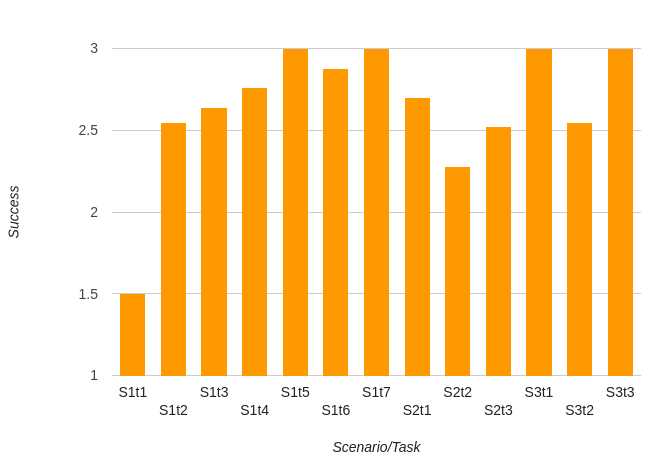
\includegraphics[width=0.9\linewidth]{help-required}
	\caption{This shows the level of help required for a particular scenario/task. If a participant required a lot of help to complete they were given a success score of 0. If they accomplished the task without any help at all they were given a score of 3. The results graphed here is the mean of all participants.}
	\label{fig:help-required}
\end{figure}

\subsection{System Usability Study Questionnaire}
\label{sub:system_usability_study_questionnaire}

The results from the usability study are divided into two distinct groups. The first group as seen in Table~\ref{tab:sus_high} has a very high SUS score. This places the interface at an usability grade of around A-B\footnote{Notes about interpreting SUS scores can be found in this article: \url{http://www.measuringu.com/sus.php}}, which is the indicator of a very usable interface. Scores of 80 and above are usually the point where users are likely to recommend a product to a friend. These scores could be affected by the backgrounds of the two participants as one had an existing understanding of provenance and the other frequently did data analysis activities such as data mining. 

However there is a second group of much lower scores as seen in Table~\ref{tab:sus_low}, placing the interface at a much lower usability grade. After further analysis of the participants and their interviews it seems that the results may be contributed to lack of sleep in on instance and difficulties interpreting questions in another. User five is the most interesting case because they completed all the tasks without any prompting and still gave the interface an unusually low score of 52.5. I believe this may be because they found some bugs related to how the undo/redo function works and this may have tainted their result.

Overall it is promising to see such high scores from the SUS questionnaire. After implementing some of the user requested features above and fixing the undo/redo bug it would be interesting to see how ProvOwl would score on a larger cohort.

\begin{table}[h]
	\centering
	\def\arraystretch{1.5}
	\caption{This higher scoring group can be contributed to the users backgrounds.}
	\label{tab:sus_high}
	\begin{tabu} to \textwidth {|c|c|X[l]|}
		\hline
		\textbf{User}&\textbf{Score}&\textbf{Notes} \\
		\hline
		\hline
		1 & 75 & Background in IT research, frequently explores and mines information on a daily basis. Logs information about themselves.\\
		2 & 85 & Strong understanding of digital provenance.\\\hline
	\end{tabu}
\end{table}

\begin{table}[h]
	\centering
	\def\arraystretch{1.5}
	\caption{This lower scoring group seems to be contributed to a number of reasons.}
	\label{tab:sus_low}
	\begin{tabu} to \textwidth {|c|c|X[l]|}
		\hline
		\textbf{User}&\textbf{Score}&\textbf{Notes} \\
		\hline
		\hline
		3 & 40 & User was tired (complained about lack of sleep) and sped through the tasks without much thought \\
		4 & 55 & English was a secondary language, participant had difficulty understanding the explanation of provenance, this also affected their ability to interpret questions. \\
		5 & 52.5 & Was very competent in use of the application and completed all tasks without prompting. They found some bugs in ProvOwl perhaps influencing their score.\\
		\hline
	\end{tabu}
\end{table}
